% chap5.tex (Definitions, Theorem and Proof)

\chapter{Real Data Analysis}
\section{Real Data Exploration}
\subsection{Data Source and Preparation}
In this chapter, we apply our proposed method to real-life data as an illustration. For instance, as a statistical consultant or data scientist, you are tasked to provide statistical advice on how to estimate the salary of a particular player in a baseball team by prediction. The baseball team in question does not want to suggest a salary that is too high or too low. However, they know some of the characteristics of a previous team that influences their salary structure but would like an objective way of estimating the current and future salaries. The goal, therefore, is to develop accurate confidence bound estimates that can be used to determine a value within these bounds that can be used to predict a player's salary on the basis of the previous team's characteristics. Using data which provides information on Major League Baseball from the 1986 and 1987 seasons by Hitters, sourced from \url{http://lib.stat.cmu.edu/datasets/baseball.data} and also available from the ISLR package in R. The StatLib library at Carnegie Mellon University was the original host of this data set, which was also used in the 1988 ASA Graphics Section Poster Session.  Essentially, this salary data was originally from Sports dated April 20, 1987, which captured excerpts on the 1986 and career statistics which were obtained from The 1987 Baseball Encyclopedia Update published by Collier Books, Macmillan Publishing Company, New York.\citep{james2017data}.

The data contains the 1987 annual salary of baseball players (in thousands of dollars) on the opening day of the season. It has 263 rows (observations) and 25 columns (variables). A brief description of the variables is provided in Table \ref{table:Data}

\vspace{0.1in}
\begin{table}[H]
	\caption{1987 Baseball Salary Data for Hitters}
	\vspace{0.1in}
	\centering
	\begin{tabular}{|p{3cm}|p{11cm}|}
		\hline
		Variable  &Description\\
		\hline
		name &	hitter's name\\
		bat86&  number of times at bat in 1986\\
		hit86&  number of hits in 1986\\
		hr86&  number of home runs in 1986\\
		run86&   number of runs in 1986\\
		rb86&  number of runs batted in in 1986\\
		wlk86& number of walks in 1986\\
		yrs&  number of years in the major leagues\\
		batcr&    number of times at bat during his career\\
		hitcr&  number of hits during his career\\
		hrcr&   number of home runs during his career\\
		runcr&    number of runs during his career\\
		rbcr&    number of runs batted in during his career\\
		wlkcr&    number of walks during his career\\
		leag86&    player's league at the end of 1986\\
		div86&    player's division at the end of 1986\\
		team86&    player's team at the end of 1986\\
		pos86 &   player's position(s) in 1986\\
		puto86 &    number of put outs in 1986\\
		asst86 &  number of assists in 1986\\
		err86 &  number of errors in 1986\\
		salary  &  1987 annual salary on opening day in thousands of  dollars\\
		leag87  &  player's league at the beginning of 1987\\
		team87  &  player's team at the beginning of 1987\\
		\hline
	\end{tabular}
	\label{table:Data}
\end{table}
Data preparation and validation were carried out. First, a salary which is the response variable was transformed through log-transformation to make it less skewed. Again highly concentrated categorical and string independent variables such as name, team86, team 87, and pos86  were removed and less concentrated ones were recoded into 0's and 1's for further analysis.

\subsection{Obtaining the best Tree from the data set}
\begin{figure}[H]
	\centering
	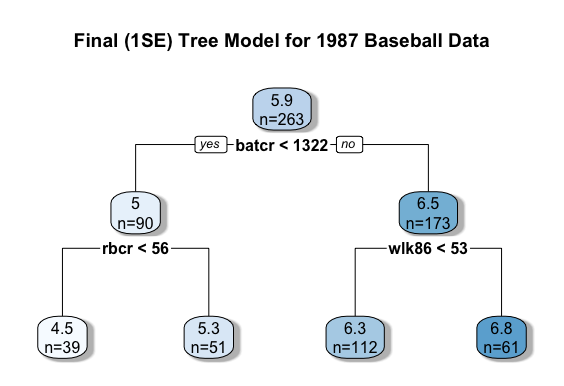
\includegraphics[scale=0.60, angle=0]{RealD_Tree.png}
	\caption{Plot of the best tree via pruning and cross validation. 
		\label{RealTree}}
\end{figure}
Using the prepared data and the CART function. Tree analysis was performed through pruning and cross-validation. By the 1-SE rule \citep{breiman1984classification},  the best tree was obtained as plotted in Fig( \ref{RealTree}).


\subsection{Estimates of  $s_t $ and $s_t^{c} $ from the best tree}
\vspace{0.1in}
\begin{table}[H]
	\caption{Table values of $s_t$ and  $s^{''}_t$ using the baseball salary data.}
	\vspace{0.1in}
	\centering
	\begin{tabular}{|p{1cm}|p{1cm}|p{2cm}| p{2cm}|p{2cm}|p{2cm}|}
		\hline
		node  &n &$\bar{y}_{t}$ &$s_t$  &Bias & $s^{''}_t$\\
		\hline
		3&	39&	4.548878&	0.2439172&	0.03598723&	0.2799044
\\
		4&	51&	5.283612&	0.3136554&	0.06161825&	0.3752736
\\
		6&	112&	6.256974&	0.4964537&	0.07495183&	0.5714055\\

		7&	61&	6.81953&	0.4862067&	0.08187276&	0.5680795\\
		\hline
	\end{tabular}
	\label{table:Baseball}
\end{table}


Also, we applied the proposed BBC method with $B=500$ bootstrap samples to estimate the biases and obtain the bias-corrected SD ($s_t^{''}$) for each of the four terminal nodes. The results are tabulated in Table \ref{table:RealD_CI}.

%We extracted the naive SD ($s_t$) from the summary of the best tree. Again with our baseball data set we generated $B=500$ bootstrap samples, with the aim of estimating SD bootstrap estimates leading to the derivation of the biased component in order to obtain the bootstrap bias-corrected SD ($s_t^{c}$). All estimates such as the naive SD ($s_t$), the bias, and the Bootstrap Biased Corrected SD ($s_t^{c}$) for all the four terminal nodes of the best tree are indicated in Table (\ref{table:Baseball})

\subsection{Empirical Coverage from the best tree}
\vspace{0.1in}
\begin{table}[H]
	\caption{Confidence  estimates of the mean  salary via BBC: $\bar{y}_t \pm z_{1-\alpha/2} s^{''}_t /\sqrt{n_t}$ }
	\vspace{0.1in}
	\begin{tabular}{ |p{1cm}|p{1cm}|p{2cm}|p{2cm}| p{2cm}|p{2cm}|p{2cm}|p{2cm}|p{2cm}|}
		\hline
		node  &n   &$\bar{y}_{t}$ &	$L_{\bar{y}_{t}}$ &$U_{\bar{y}_{t}}$ & $e^{\bar{y}_{t}}$ & $L_{e^{\bar{y}_{t}}}$&$U_{e^{\bar{y}_{t}}}$\\
		\hline
		3&	39&	4.548878&	4.461031&	4.636724&	94.52626&	86.57672&	103.2057
\\
		4&	51&	5.283612&	5.180618&	5.386605&	197.08035&	177.79261&	218.4605
\\
		6&	112&	6.256974&	6.151151&	6.362798&	521.6383&	469.257	&579.8667
\\
		7&	61&	6.81953&	6.676972&	6.962089&	915.55493&	793.91162&	1055.8365\\
		\hline
	\end{tabular}
	\label{table:RealD_CI}
\end{table}
Table (\ref{table:RealD_CI}) show the 95\% confidence interval for the node mean using our bias-corrected SD for all terminal nodes obtained from the best tree through our proposed method BBC: $\bar{y}_t \pm z_{1-\alpha/2} s^{''}_t /\sqrt{n_t}$ ,where  alpha was chosen to be $\alpha=0.05$, $n_t$ is the total number of samples in  each individual terminal node, $\bar{y}_{t}$ is logsalary (log of the mean salary) and $s_t^{''}$ is the BBC SD estimates for each terminal node. For better interpretability, confidence intervals for mean salary on its original scale are also obtained by taking the exponential. These are also shown in Table \ref{table:RealD_CI}.  

\vspace{0.1in}
\vspace{0.1in}
\begin{figure}[H]
	\centering
	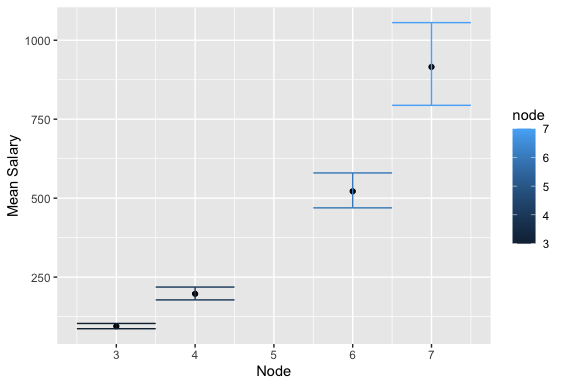
\includegraphics[scale=0.70, angle=0]{Conf_Plot.png}
	\caption{Plot of the Confident Estimates of the Mean Salary}. 
		\label{Conf_Plot}
\end{figure}
%\vspace{0.1in}
Figure(\ref{Conf_Plot}) is an error bound plot depicting table (\ref{table:RealD_CI}) estimates ( $L_{e^{\bar{y}_{t}}}$, $U_{e^{\bar{y}_{t}}}$) graphically. Node 3 defines a group of players who have the lowest average salary. These players are characterized by the number of bats less than 1322 and the number of runs batted less than 56 in their career. Node 7 is characterized by players with the number of bats greater than 1322 and number of walks in 1986 greater than 53 in career having the highest average salary.



